%!TEX root = ../thesis.tex
\begin{section}{General assumptions}
\label{sec:1D_introduction}

We consider a forager in one dimension by first defining the search space as the set of all real numbers, $\mathbb{R}$.
That is, the forager can search anywhere along a single dimension.
Targets are equispaced along this search space, a distance of $\lambda$ apart.
\cref{fig:1dmodels:searchspace} shows what this scenario may look like.

\usetikzlibrary{shapes.misc}
\tikzset{cross/.style={cross out, draw=black, minimum size=2*(#1-\pgflinewidth), inner sep=0pt, outer sep=0pt},
	cross/.default={4pt}}
\begin{figure}[H]
	\centering
	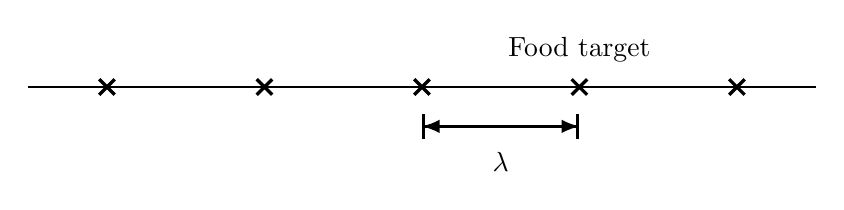
\begin{tikzpicture}
	\draw (-5,0) -- (5,0) ; %Draws the big line
	\foreach \x in  {-4,-2,0,2,4}
	\draw[shift={(\x,0)},color=black] node[cross,very thick] {}; %Puts a cross at x = -6,-2,2,6
	\draw[|-latex,very thick] (0,-0.5) -- (2,-0.5) ; %draws the lambda line with left arrow
	\draw[latex-|,very thick] (0,-0.5) -- (2,-0.5) ; %draws the lambda line with right arrow
	\draw (1,-1.2) node[above]{$\lambda$}; %labels the lambda line
	\draw (2,0.2) node[above]{Food target}; %labels the third from left cross.
	\end{tikzpicture}
	\caption[The full search space for the one-dimensional model]{The search space for the one-dimensional foraging model.
	Food patches (crosses) are deterministically spaced along the search space, a distance of $\lambda$ apart.
	\label{fig:1dmodels:searchspace}}
\end{figure}

In reality, food patches will not usually be distributed deterministically and so more realistic one-dimensional models would allow food patches to be distributed along $\mathbb{R}$ according to some probability distribution.
Our assumption of deterministically spaced patches makes solving for the search efficiency easier, and we investigate the effects of making this assumption in \cref{sec:1D_assumptions:deterministic_targets}.

Two types of food patch behaviours are considered: \emph{destructive foraging}, in which the target is destroyed after the forager reaches it, and \emph{non-destructive foraging}, in which the target is not destroyed and can be revisited an unlimited number of times.

Our model assumes that the forager has a radius of vision, $r_v$, with which it can sense any targets that are within $r_v$ of its location.
After a target enters the forager's radius of vision, the forager moves directly to the target.
Initially, we consider a model where the forager has a constant radius of vision, but eventually extend our results in \cref{sec:1dMMRW} to allow the radius of vision to switch based on the state of an underlying Markov chain.

The forager's movement along the $x$-axis is governed by a random process.
In \cref{sec:1dRW}, we consider a strategy in which the forager uses a random walk, with a general step-length distribution.
This is extended to a Markov-modulated random walk strategy in \cref{sec:1dMMRW}.
We are interested only in discrete-time random processes, in which the forager takes discrete ``steps''.
Our notion of a step corresponds to a ``reorientation'' step, in which the animal decides which direction and for what distance it should travel for its next movement, rather than steps representing physical steps made by the forager.
We also disallow the forager from jumping over or skipping targets, and any step that would cause this to occur is truncated.
In one dimension, this assumption is perfectly valid, as there is no way that an animal can pass a target without it at one point being at the target itself.

Our primary aim is to determine the most efficient foraging strategy, where the efficiency is given by
\begin{equation*}
\eta = \frac{1}{\E{L}},
\end{equation*}
where $L$ is the total distance travelled to find the first food patch.
This notion of efficiency is common throughout the literature (e.g \cite{Bartumeus_2013,Viswanathan_1999}) and only considers the distance required to find a single patch.
However, in the case of destructive foraging the food patches are becoming more sparse over time, and so we would expect the efficiency to be decreasing over time.
Because of this, we investigate this notion of efficiency and compare it with others in \cref{sec:1D_assumptions:efficiency}.

Since we are only considering the distance travelled to find a single patch, we can reduce the search space to $[0,\lambda]$, where the two ends of this interval correspond to the targets.
\cref{fig:1dmodels:searchinterval} shows what this new model looks like.
In the reduced model, the assumption of destructive targets corresponds to a search that starts at $\lambda/2$, and that of non-destructive targets corresponds to a search that starts at $r_v$.
This choice of starting locations has been used throughout the literature (e.g. \cite{Bartumeus_2013,}), although we put this on more rigorous grounding in \cref{sec:1D_assumptions:efficiency}.
For now, we provide a brief intuitive explanation of why this is the case.
For a non-destructive forager, after reaching a target and beginning a new search, the target it just found is still available and so its search is beginning right next to a target, at $r_v$.
For a destructive forager, without loss of generality assume that it finds the target at $0$.
Then, for its next search the two nearest patches are at $-\lambda$ and $\lambda$, and its location is halfway between them at $0$.
After scaling this becomes equivalent to starting at $\lambda/2$ on the interval $[0,\lambda]$.

\begin{figure}[H]
	\centering
	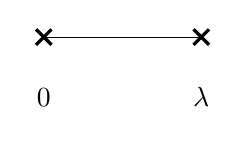
\begin{tikzpicture}
		\draw (-1,0) -- (1,0) ; %Draws the big line
		\foreach \x in  {-1,1}
		\draw[shift={(\x,0)},color=black] node[cross,very thick] {}; %Puts a cross
		\draw (-1.0,-1.0) node[above]{$0$}; %labels endpoint
		\draw (1.0,-1.0) node[above]{$\textcolor{black}{\lambda}$}; %labels endpoint
	\end{tikzpicture}
	\caption[The reduced search space for the one-dimensional model]{The search space for a single search, which without loss of generality is the interval $[0,\lambda]$.
	The two food patches are at $x=0$ and $x=\lambda$.
	\label{fig:1dmodels:searchinterval}}
\end{figure}

To determine the efficiency of a search, we shall first derive an expression for $\E{L}$.
Although the overall aim is to determine an expression for the efficiency, we are also interested in determining other quantities for a search, such as the total number of steps taken.
The derivation of many of these quantities is similar in structure, so rather than showing each separately, we first derive the total ``cost'' of a strategy, based on some general cost function for each step.
Using this result, we can determine the efficiency and the total steps taken, among other things, with relative ease.

The derivation of the efficiency of the random walk strategy comes mostly from Bartumeus \etal \cite{Bartumeus_2013}, although some of the results were first found outside of the context of animal foraging \cite{Buldyrev_2001_avetime,Buldyrev_2001_prop}.
The reason for including the derivation in this thesis is twofold.

First, the derivation for the Markov-modulated random walk is fairly similar in structure to that of the random walk strategy.
Some of the techniques that are used require conditions that, while not obvious in the Markov-modulated random walk case, are quite obviously true in the case of the random walk.
Because of this, the paper by Bartumeus \etal \cite{Bartumeus_2013} does not give these details for the random walk strategy.
In particular, applying the Dirac delta function (\cref{thm:1dRW_cost:EV_dirac}) and showing the fact that the operator norm is less than unity (\cref{thm:1dRW_cost:Q_operator_norm}) are not treated by Bartumeus \etal \cite{Bartumeus_2013}.
We include these details that were missed as they help make the derivation for the Markov-modulated case clearer.
Our notation is also reasonably different from Bartumeus \etal \cite{Bartumeus_2013} in order to maintain consistency between the unmodulated and modulated strategies.

Second, the random walk strategy is simple enough to allow us a good insight into why many of the model assumptions are needed, and how relaxing any of these may be difficult.
The notation becomes more complex when Markov-modulation is considered, and much of the intuition is lost.
\end{section}
